\documentclass[12pt,a4paper]{article}
\usepackage[UTF8,fontset=none]{ctex}
\setCJKmainfont{Noto Sans CJK SC}[AutoFakeBold]
\setCJKsansfont{Noto Sans CJK SC}
\setCJKmonofont{Noto Sans Mono CJK SC}
\usepackage[margin=2cm,top=2.2cm,bottom=2.2cm]{geometry}
\usepackage{graphicx}
\usepackage{booktabs}
\usepackage{hyperref}
\usepackage{listings}
\usepackage{xcolor}
\usepackage{enumitem}
\usepackage{fontspec}
\usepackage{tikz}
\usepackage{tabularx}
\usetikzlibrary{shapes.geometric, arrows.meta, positioning, calc}

\hypersetup{
  colorlinks=true,
  linkcolor=blue!70!black,
  urlcolor=blue!70!black,
  citecolor=blue!70!black
}

\lstset{
  basicstyle=\ttfamily\scriptsize,
  breaklines=true,
  frame=single,
  backgroundcolor=\color{gray!5},
  keywordstyle=\color{blue!70!black},
  commentstyle=\color{green!50!black},
  stringstyle=\color{red!60!black},
  columns=fullflexible,
  keepspaces=true,
  xleftmargin=2pt,
  xrightmargin=2pt,
}

\definecolor{brand}{RGB}{99,102,241}
\definecolor{brandlight}{RGB}{238,242,255}

\title{\vspace{-1em}{\textbf{Noteworthy}}\\[4pt]
{\large 轻量化在线笔记应用 --- 项目说明文档}\\[2pt]
{\small\color{gray} 前后端分离 \textbullet\ 富文本编辑 \textbullet\ JWT 认证 \textbullet\ 响应式设计}}
\author{
  姓名：XXX \quad 学号：XXXXXXXX \\[2pt]
  选题方向：Web 全栈应用开发
}
\date{\today}

\begin{document}
\maketitle
\thispagestyle{empty}
\tableofcontents
\newpage

% ============================================================
\section{项目基本信息}
% ============================================================

\begin{itemize}[leftmargin=1.5em,itemsep=2pt]
  \item \textbf{项目名称}：Noteworthy --- 轻量化在线笔记软件
  \item \textbf{选题方向}：Web 全栈应用开发
  \item \textbf{作者}：XXX \quad \textbf{学号}：XXXXXXXX
\end{itemize}

\subsection{运行方式}

\textbf{前置依赖}：Docker \& Docker Compose、Python 3.10+、Node.js 18+

\begin{enumerate}[itemsep=2pt]
  \item \textbf{启动数据库}：\lstinline|docker compose up -d db|
  \item \textbf{启动后端}：
\begin{lstlisting}[language=bash]
cd backend && cp .env.example .env
python3 -m venv venv && source venv/bin/activate
pip install -r requirements.txt && alembic upgrade head
uvicorn app.main:app --reload --host 0.0.0.0 --port 8000
\end{lstlisting}
  访问 \url{http://localhost:8000/docs} 查看 Swagger API 文档。
  \item \textbf{启动前端}：
\begin{lstlisting}[language=bash]
cd frontend && npm install && npm run dev
\end{lstlisting}
  浏览器打开 \url{http://localhost:5173} 即可使用。
\end{enumerate}

% ============================================================
\section{产品概述}
% ============================================================

\subsection{产品定位}

Noteworthy 定位为\textbf{轻量化、高可用的在线笔记平台}，面向个人知识管理场景，提供从采集、组织到检索的完整笔记工作流。与同类产品相比，其核心差异化优势在于：

\begin{itemize}[leftmargin=1.5em,itemsep=1pt]
  \item \textbf{全栈自研}：前后端完全自主开发，无第三方笔记服务依赖，数据主权可控。
  \item \textbf{专业编辑体验}：基于 ProseMirror 内核的 Tiptap 编辑器，支持 15+ 富文本扩展、代码语法高亮与图片上传，编辑能力远超 Markdown 纯文本方案。
  \item \textbf{企业级安全}：BCrypt(12 rounds) 密码哈希 + JWT 双令牌无感续期 + 用户级数据隔离，安全机制对标生产环境标准。
  \item \textbf{智能资源管理}：双层图片清理策略（即时 + 定时兜底）与归档笔记自动过期，解决服务器存储泄漏问题。
\end{itemize}

\subsection{功能全景}

\begin{table}[h]
\centering
\small
\begin{tabularx}{\textwidth}{lX}
\toprule
\textbf{功能域} & \textbf{能力描述} \\
\midrule
用户认证 & 注册/登录、JWT 双令牌鉴权、令牌自动刷新、导航守卫 \\
笔记本管理 & 创建/重命名/删除、自定义图标与颜色、拖拽排序、归档 \\
笔记编辑 & Tiptap 富文本（15+ 扩展）、3s 防抖自动保存、\texttt{Ctrl+S} 手动保存、字数统计 \\
笔记组织 & 置顶、归档/恢复、标签多对多关联、跨笔记本聚合视图 \\
图片系统 & 上传（$\leq$5\,MB，5 种格式）、即时孤立清理 + 定时全量扫描、归档 $>$7\,天自动删除 \\
全文搜索 & 标题 + 纯文本 ILIKE 模糊匹配、按笔记本过滤、分页 \\
UI/UX & 玻璃拟态设计、深色模式、响应式三端适配、骨架屏 + Toast + 页面过渡动画 \\
\bottomrule
\end{tabularx}
\end{table}

% ============================================================
\section{技术架构}
% ============================================================

\subsection{技术选型与决策}

\begin{table}[h]
\centering
\small
\begin{tabularx}{\textwidth}{llX}
\toprule
\textbf{层面} & \textbf{技术} & \textbf{选型理由} \\
\midrule
前端框架 & Vue 3 + TS & Composition API + \texttt{<script setup>} 简洁高效；TypeScript 全量类型覆盖 \\
构建工具 & Vite 6 & 原生 ESM HMR，冷启动 $<$300\,ms，较 Webpack 提升 10--100$\times$ \\
状态管理 & Pinia & Vue 3 官方推荐，Setup Stores 与 Composition API 风格统一，TS 推导完善 \\
样式方案 & UnoCSS & 原子化按需生成，零运行时开销；兼容 Tailwind 生态 \\
富文本 & Tiptap & ProseMirror 内核，可扩展架构支持表格/代码高亮/任务列表等企业级功能 \\
后端框架 & FastAPI & async/await 原生、自动 OpenAPI 文档、Pydantic v2 校验性能提升 5--50$\times$ \\
ORM & SQLAlchemy 2.0 & 声明式映射 + \texttt{select()} 风格 + 异步引擎，2.0 重写后类型提示完备 \\
数据库 & PostgreSQL 16 & JSONB 原生存储 Tiptap 文档、\texttt{pg\_trgm} 三字符索引加速模糊搜索 \\
认证 & JWT 双令牌 & Access(30\,min) + Refresh(7\,d)，无状态鉴权，水平扩展友好 \\
容器化 & Docker Compose & \texttt{postgres:16-alpine} 镜像，\texttt{healthcheck} 就绪探针保障启动顺序 \\
\bottomrule
\end{tabularx}
\end{table}

\subsection{系统架构}

后端采用\textbf{四层分离}架构，严格遵循单一职责原则：

\begin{center}
\begin{tikzpicture}[
  layer/.style={rectangle, draw, rounded corners=3pt, minimum width=11cm, minimum height=0.85cm, align=center, font=\small},
  >=Stealth,
  node distance=0.35cm
]
  \node[layer, fill=blue!8]   (route) {Router 层 --- HTTP 请求处理、参数校验、依赖注入};
  \node[layer, fill=green!8,  below=of route] (service) {Service 层 --- 业务逻辑、权限校验、数据编排};
  \node[layer, fill=orange!8, below=of service] (repo) {Repository 层 --- 泛型 CRUD、分页查询、数据访问抽象};
  \node[layer, fill=red!8,    below=of repo] (model) {Model 层 --- SQLAlchemy ORM 映射、关系定义、约束声明};

  \draw[->, thick] (route) -- (service);
  \draw[->, thick] (service) -- (repo);
  \draw[->, thick] (repo) -- (model);
\end{tikzpicture}
\end{center}

前端按功能域组织：\textbf{API 模块}封装接口调用与令牌刷新拦截器，\textbf{Pinia Store}管理响应式状态，\textbf{View}负责声明式渲染，\textbf{UI 组件库}提供一致的设计系统。

\subsection{数据模型}

系统共 5 张表，核心实体关系如下：

\begin{center}
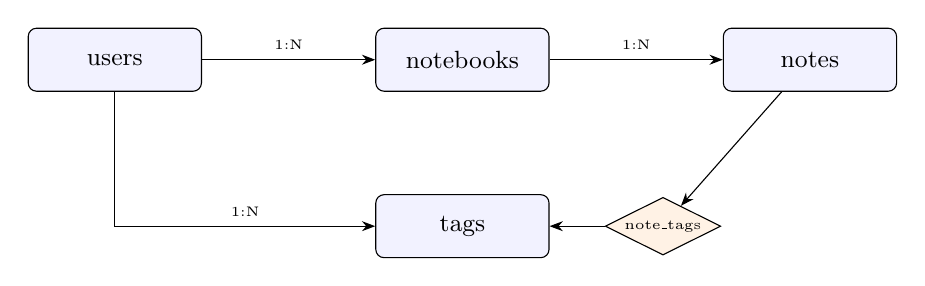
\begin{tikzpicture}[
  entity/.style={rectangle, draw, rounded corners=3pt, minimum width=2.2cm, minimum height=0.8cm, align=center, fill=blue!5, font=\small},
  rel/.style={diamond, draw, aspect=2, fill=orange!10, inner sep=1pt, font=\tiny},
  >=Stealth,
  every edge/.style={draw, ->},
  node distance=1.6cm and 2.2cm
]
  \node[entity] (user) {users};
  \node[entity, right=of user] (notebook) {notebooks};
  \node[entity, right=of notebook] (note) {notes};
  \node[entity, below=1.3cm of notebook] (tag) {tags};
  \node[rel, right=0.7cm of tag] (nt) {note\_tags};

  \draw[->] (user) -- node[above, font=\tiny]{1:N} (notebook);
  \draw[->] (notebook) -- node[above, font=\tiny]{1:N} (note);
  \draw[->] (user) |- node[near end, above, font=\tiny]{1:N} (tag);
  \draw[->] (note) -- (nt);
  \draw[<-] (tag) -- (nt);
\end{tikzpicture}
\end{center}

\begin{table}[h]
\centering
\scriptsize
\begin{tabularx}{\textwidth}{llX}
\toprule
\textbf{表} & \textbf{关键字段} & \textbf{设计要点} \\
\midrule
users & id(UUID), username, email, hashed\_password & UUID 主键防枚举；username/email 唯一索引 \\
notebooks & id, user\_id(FK), name, icon, color, sort\_order & CASCADE 级联删除笔记；sort\_order 支持自定义排序 \\
notes & id, notebook\_id(FK), user\_id(FK), content(JSONB), plain\_text, is\_pinned, is\_archived & JSONB 存储 Tiptap 文档；plain\_text 冗余字段加速搜索 \\
tags & id, user\_id(FK), name, color & (user\_id, name) 联合唯一约束防重复 \\
note\_tags & note\_id(PK), tag\_id(PK) & 多对多关联表，双主键 + CASCADE \\
\bottomrule
\end{tabularx}
\end{table}

% ============================================================
\section{核心功能实现}
% ============================================================

\subsection{JWT 双令牌认证}

\begin{enumerate}[leftmargin=1.5em,itemsep=2pt]
  \item \textbf{签发}：登录成功后签发 Access Token（30\,min）与 Refresh Token（7\,d），均使用 HS256 算法，payload 含 \texttt{sub}/\texttt{iat}/\texttt{exp}/\texttt{type} 声明。
  \item \textbf{鉴权}：请求经 \texttt{get\_current\_user} 依赖注入解析 Access Token，校验 \texttt{type="access"} 及有效期，注入用户对象至路由函数。
  \item \textbf{无感续期}：前端 Axios 响应拦截器捕获 401 后，以 Refresh Token 调用 \texttt{/auth/refresh} 获取新令牌对。\textbf{并发控制}：首个 401 触发刷新，其余请求入队等待，刷新完成后统一重试，避免竞态导致 Token 失效。
  \item \textbf{数据隔离}：所有 Service 层查询均携带 \texttt{user\_id} 条件，确保用户间数据物理隔离。
\end{enumerate}

\subsection{富文本编辑器}

基于 Tiptap（ProseMirror 内核）构建，集成 15+ 扩展：

\noindent\begin{minipage}[t]{0.48\textwidth}
\begin{itemize}[leftmargin=1em,itemsep=0pt,font=\scriptsize]
  \item StarterKit（段落/标题/列表/引用/代码）
  \item CodeBlockLowlight（lowlight 语法高亮）
  \item Table + TableRow/Cell/Header
  \item TaskList + TaskItem（嵌套）
  \item Image（服务端上传，非 Base64）
\end{itemize}
\end{minipage}\hfill
\begin{minipage}[t]{0.48\textwidth}
\begin{itemize}[leftmargin=1em,itemsep=0pt,font=\scriptsize]
  \item TextStyle + Color（16 色预设 + 拾色器）
  \item Highlight / Underline / Link
  \item Typography / Placeholder
  \item CharacterCount（实时字数统计）
  \item 自定义 CodeBlockWithLabel（语言标签）
\end{itemize}
\end{minipage}

\vspace{4pt}
\textbf{保存策略}：编辑器 \texttt{onUpdate} 触发 3\,s 防抖定时器，标题变更同样触发；\texttt{Ctrl+S} 立即保存；组件卸载时若 \texttt{isDirty} 则兜底保存。状态栏三态指示：\textcolor{green!60!black}{\textbf{Saved}} / \textcolor{orange!80!black}{\textbf{Unsaved}} / \textcolor{yellow!80!orange}{\textbf{Saving...}}。

\subsection{图片生命周期管理}

\begin{enumerate}[leftmargin=1.5em,itemsep=2pt]
  \item \textbf{上传}：\texttt{POST /uploads/images}，校验 Content-Type（JPEG/PNG/GIF/WebP/SVG）与大小（$\leq$5\,MB），UUID 重命名存储至 \texttt{uploads/}，返回 \texttt{/uploads/<filename>} URL。
  \item \textbf{即时清理}：笔记更新时 diff 新旧 content 中的图片引用集合，删除不再被引用的文件；笔记删除时同步清理关联图片。
  \item \textbf{定时兜底}：后台 \texttt{cleanup\_loop} 每小时全量扫描：(a) 删除 \texttt{uploads/} 中未被任何 note 引用的文件；(b) 删除 \texttt{archived\_at} 超过 7 天的归档笔记及其标签关联。
\end{enumerate}

\subsection{全文搜索}

笔记创建/更新时，后端递归遍历 Tiptap JSON 提取 \texttt{type="text"} 节点，拼接为 \texttt{plain\_text} 冗余字段。搜索接口基于 \texttt{ILIKE} 对 \texttt{title} 和 \texttt{plain\_text} 进行模式匹配，支持按 \texttt{notebook\_id} 过滤与分页。数据库初始化时已启用 \texttt{pg\_trgm} 扩展，可平滑升级为三字符索引加速。

% ============================================================
\section{技术挑战与解决方案}
% ============================================================

\textbf{挑战 1：JWT 并发刷新竞态}。SPA 中多个异步请求同时收到 401 时，若各自独立刷新令牌，后到的刷新请求会使先前的 Refresh Token 失效。\textbf{方案}：在 Axios 拦截器中实现\textbf{请求队列}模式——设置 \texttt{isRefreshing} 互斥标志，首个 401 持有刷新权，其余以 Promise 入队；刷新成功后 \texttt{processQueue(null, newToken)} 统一重试，失败则全部拒绝并登出，O(1) 额外开销。

\textbf{挑战 2：服务器图片存储泄漏}。用户删除笔记或移除图片后，文件系统残留无人引用的图片。\textbf{方案}：双层清理——(1) \textbf{即时层}：\texttt{NoteService.update/delete} 中 diff 新旧 content 图片集合，立即删除孤立文件；(2) \textbf{兜底层}：\texttt{cleanup\_loop} 每小时全量扫描，删除无主文件与归档超 7 天的笔记。两层互补确保零泄漏。

% ============================================================
\section{项目结构与 API}
% ============================================================

\begin{lstlisting}[language={}]
WebProgram/
+-- docker-compose.yml          # PostgreSQL 16 (alpine)
+-- docker/init.sql             # uuid-ossp + pg_trgm
+-- backend/app/
|   +-- main.py                 # FastAPI app factory & lifespan
|   +-- api/v1/                 # Routers (auth, notebooks, notes, tags, search, uploads)
|   +-- core/                   # config, security, database, exceptions
|   +-- models/                 # ORM (User, Notebook, Note, Tag, NoteTag)
|   +-- schemas/                # Pydantic v2 schemas
|   +-- services/               # Business logic + cleanup
|   +-- repositories/           # Generic BaseRepository CRUD
+-- frontend/src/
|   +-- api/                    # Axios client + refresh interceptor
|   +-- components/{ui,layout}  # Design system + layout
|   +-- layouts/                # DefaultLayout, AuthLayout
|   +-- router/                 # Vue Router + authGuard
|   +-- stores/                 # Pinia (auth, notes, notebooks, tags, editor, ui)
|   +-- views/                  # 10 page views
+-- docs/                       # Project documentation
\end{lstlisting}

后端采用\textbf{路由 $\to$ 服务 $\to$ 仓库 $\to$ 模型}四层架构，前端按功能域组织。系统共暴露 16 个 API 端点：

\begin{table}[h]
\centering
\scriptsize
\begin{tabularx}{\textwidth}{llX}
\toprule
\textbf{方法} & \textbf{路径} & \textbf{说明} \\
\midrule
POST & /api/v1/auth/register & 用户注册，返回双令牌 \\
POST & /api/v1/auth/login & 登录，BCrypt 校验 \\
POST & /api/v1/auth/refresh & 刷新令牌对 \\
GET  & /api/v1/auth/me & 当前用户信息 \\
GET/POST & /api/v1/notebooks & 笔记本列表/创建 \\
GET/PUT/DELETE & /api/v1/notebooks/\{id\} & 笔记本 CRUD \\
GET/POST & /api/v1/notebooks/\{id\}/notes & 笔记列表/创建 \\
GET/PUT/DELETE & /api/v1/notes/\{id\} & 笔记 CRUD \\
PATCH & /api/v1/notes/\{id\}/pin & 置顶/取消 \\
PATCH & /api/v1/notes/\{id\}/archive & 归档/恢复 \\
POST/DELETE & /api/v1/notes/\{id\}/tags & 附加/移除标签 \\
GET/POST & /api/v1/tags & 标签列表/创建 \\
PUT/DELETE & /api/v1/tags/\{id\} & 标签更新/删除 \\
GET  & /api/v1/search?q=\textit{kw} & 全文搜索 \\
POST & /api/v1/uploads/images & 图片上传 \\
\bottomrule
\end{tabularx}
\end{table}

% ============================================================
\section{学习总结与自我评估}
% ============================================================

\subsection{学习收获}

\begin{itemize}[leftmargin=1.5em,itemsep=0pt]
  \item 掌握前后端分离全栈开发完整流程：ER 设计、Alembic 迁移、RESTful API、SPA 交互。
  \item 深入理解 JWT 认证体系：双令牌策略、并发刷新队列、依赖注入鉴权、数据隔离。
  \item 实践 ProseMirror 文档模型：Tiptap 扩展机制、JSONB 存储、纯文本提取与搜索。
  \item 积累异步编程经验：SQLAlchemy 2.0 async、FastAPI async routes、asyncio 后台任务。
  \item 工程化能力提升：泛型 Repository、双层资源清理、Axios 拦截器设计。
\end{itemize}

\subsection{完成度评估}

全部 7 个功能模块均已实现（用户认证、笔记本 CRUD、笔记 CRUD、富文本编辑器、图片系统、搜索与标签、UI/UX），代码结构清晰，API 文档自动生成。

\textbf{未来演进方向}：\texttt{tsvector} 全文搜索 + GIN 索引替代 ILIKE；WebSocket 实时通知；笔记导出 Markdown/PDF；协作编辑（CRDT/OT）。

% ============================================================
\section{原创性声明与引用}
% ============================================================

本项目为个人独立完成的设计与开发作品，所有核心代码均为原创。

\textbf{主要开源依赖}：Vue 3 (\url{https://vuejs.org/})、Pinia (\url{https://pinia.vuejs.org/})、FastAPI (\url{https://fastapi.tiangolo.com/})、SQLAlchemy (\url{https://www.sqlalchemy.org/})、Tiptap (\url{https://tiptap.dev/})、UnoCSS (\url{https://unocss.dev/})、Phosphor Icons (\url{https://phosphoricons.com/})、lowlight (\url{https://github.com/wooorm/lowlight})

\end{document}
